\part{Oscilador de Wien}


\section{Introducción}

A lo largo de esta parte, se centrará en realizar un oscilador generador
de onda sinusoidal basado en el puente de \emph{Wien.} Para poder
entender este oscilador, resulta necesario comprender el criterio
de Barkhausen, el cual es imprecindible para realizar el oscilador.

\subsection{Criterio de Barkhausen}

Dado un sistema realimentado negativamente, siendo \emph{A }la ganancia
de lazo abierto y $\beta$ la ganancia de realimentación, entonces
se define $T(s)=A(s)\beta(s)$ como la ganancia de lazo de realimentación.

\begin{figure}[H]
\begin{centering}
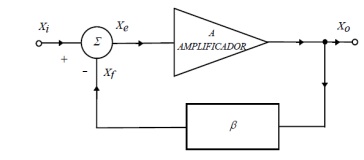
\includegraphics{../Ex1/Resources/Realimentado}
\par\end{centering}
\caption{Sistema realimentado}

\end{figure}

De acuerdo con lo desarrollado en el libro \emph{Design With Operational
Amplifiers And Analog Integrated Circuits}\footnote{\emph{A lo largo del capitulo 10.1 durante el desarrolo de Basic Wien-Bridge
Oscillator}}\emph{, }pueden ocurrir 3 posibles situaciónes para la ganancia de
lazo de realimentación \emph{T(s)}:
\begin{enumerate}
\item \emph{T($S_{0}$) < 1} : Lo cual supone una atenuación de la señal
por lo que el sistema resulta estable sin oscilar.
\item \emph{T($S_{0}$) > 1} : Lo cual genera una amplificación de la señal
resultando en un sistema inestable que con el correr del tiempo generará
que el amplificador oscile
\item \emph{T($S_{0}$) = 1} : Esta es considerada una estabilidad neutral
ya que no atenua ni amplifica la señal. Esta es la condición que se
tiene en cuenta para que el criterio funcione.
\end{enumerate}
De acuerdo con lo mencionado en el libro, para que se cumpla la condición
3, es necesario tener un par de polos conjugados sobre el eje $j\omega$.

\subsection{Oscilador de \emph{Wien}}

Dado un circuito como el que se muestra en la Figura \ref{1_1}, se
podrá calcular como se mencionó previamente, la ganancia de lazo de
realimentación. 

\begin{figure}[H]
\begin{centering}
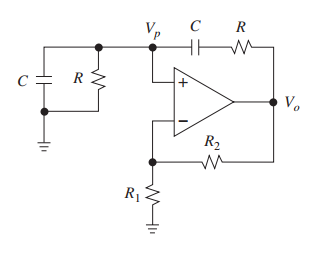
\includegraphics{../Ex1/Resources/CircuitoWien.PNG}
\par\end{centering}
\caption{Circuito de Wien}
\label{1_1}

\end{figure}

Como se menciona en el libro\footnote{Partiendo de la ecuación 10.4 y 10.5 de la pagina 486 del libro}
se llega a la ecuación mencionada a continuación:

\begin{equation}
T(f)=\frac{1+\frac{R_{2}}{R_{1}}}{3+j\left(\frac{f}{f_{0}}-\frac{f_{0}}{f}\right)}\label{eq:1_1}
\end{equation}

\begin{equation}
f_{0}=\frac{1}{2\pi RC}\label{eq:1_1_1}
\end{equation}

Por lo tanto, si se remplaza \emph{f} por la frecuencia $f_{0}$,
se obtiene

\begin{equation}
T\left(f_{0}\right)=\frac{1+\frac{R_{2}}{R_{1}}}{3}\label{eq:1_2}
\end{equation}

Consecuentemente, como se desea cumplir con la condición 3 mencionada
en la sbsección anterior, necesariamente $\frac{R_{2}}{R_{1}}=2$.
Por ende, cuando se cumpla esta condición, resulta evidente que se
generará un puente balanceado a lo largo de la frecuencia $f_{0}$.

\section{Análisis del circuito propuesto}

A lo largo de esta sección nos centraremos en analizar el circuito
propuesto por la cátedra que se puede observar en la Figura \ref{1_3}.

\begin{figure}[H]
\begin{centering}
A su vez, al calcular la distorsión armonica se obtuvo que:
\par\end{centering}
\[
THD=
\]
\begin{centering}
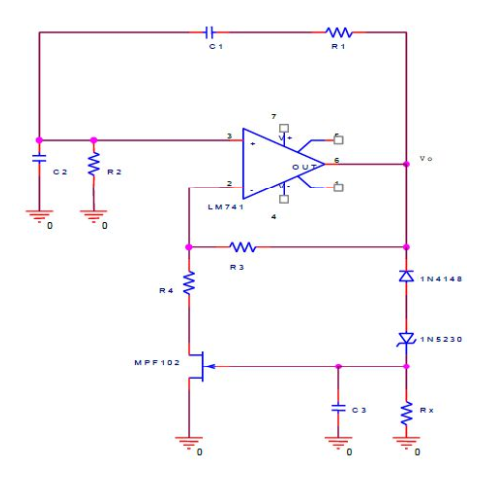
\includegraphics[scale=0.7]{../Ex1/Resources/Circuito}
\par\end{centering}
\caption{Circuito de Oscilador propuesto}
\label{1_3}

\end{figure}

Como se puede ver en la figura, el circuito propuesto es bastante
parecido al mencionado en la Figura \ref{1_1}, los componentes adicionales
agregados forman parte de lo que se llama \emph{Automatic Amplitude
Control}\footnote{Control Automático de Ganancia o CAG en español}
(AAC). El AAC, es la etapa del circuito encargada de ajustar el valor
de $\frac{R_{3}}{R_{4}}$ dinámicamente con el objetivo de suplir
las falencias constructivas de los elementos resistivos, que generan
un determinado error en el cociente, para llevarlo al valor esperado
de 2.

\subsection{\emph{Automatic Amplitude Control (AAC)\label{subsec:Automatic-Amplitude-Control}}}

\subsubsection{Transistor JFET-N}

Para poder entender el funcionamiento del AAC, es necesario primero
entender como se comporta un JFET-N, para eso, se puede observar la
Figura \ref{1_4}.

\begin{figure}[H]
\begin{centering}
\includegraphics[scale=0.4]{\string"../Ex1/Resources/ids VS vds\string".png}
\par\end{centering}
\caption{$I_{DS}$ en función de $V_{DS}$, para valores de VGS entre -3 (V)
(linea negra) y 0.5(V) (linea azul) }
\label{1_4}

\end{figure}

\begin{figure}[H]
\begin{centering}
\subfloat[Para grandes variaciones]{\begin{centering}
\includegraphics[scale=0.3]{\string"../Ex1/Resources/RDS vs VDS 1\string".png}
\par\end{centering}

}\subfloat[Para pequeñas variaciones]{\begin{centering}
\includegraphics[scale=0.3]{\string"../Ex1/Resources/RDS vs VDS 2\string".png}
\par\end{centering}

}
\par\end{centering}
\caption{$R_{DS}$en función de $V_{DS}$ para valores de $V_{GS}$ entre -2.5(V)
(linea negra) y 0.5(V) (linea verde)}
\label{1_5}

\end{figure}

Como se pudo observar en la Figura \ref{1_5}, se pude utilizar al
transisto JFET-N como resistencia variable, esto es altamente útil
para ajustar el valor del cociente $\frac{R_{3}}{R_{4}}$ visto anteriormente
y utilizarlo a nuestro favor.

\subsubsection{Diodos en serie\label{subsec:Diodos-en-serie}}

Debido a que el oscilador de wien debe poder funcionar sin señal de
entrada, se debe crear un control sobre $\frac{R_{3}}{R_{4}}$ de
modo tal que, cuando el circuito se alimente, rapidamente se llegue
a la oscilación. Esto se realiza mediante el cambo dinamico de $R_{4}$,
es decir, cuando el circuito permanezca apagado, y durante los primeros
instantes de alimentación, $R_{4}$ debe permanecer lo suficientemente
baja poara que el cociente sea lo suficientemente mayor a 2 para lograr
un tiempo de establecimiento relativamente corto, sin embargo, una
vez que se llega a ese tiempo de establecimiento, se debe procurar
de aumentar el valor de $R_{4}$ de modo tal que el cociente de resistencias
sea 2, como fue explicado anteriormente. Para lograr esto, entran
en juego los diodos, que cuando la tensión Vo es lo suficientemente
chica, los diodos no conduzcan, generando asi que el JFET tenga una
resistencia interna aproximadamente igual a 0, y cuando Vo supera
la tensión de umbral de los diodos (aproximadamente 5.4(V)), estos
conduzcan corriente, cargen el capacitor C3 y ajusten la resistencia
interna del transistor $R_{T}$ para que $\frac{R_{3}}{R_{4}+R_{T}}<2$.

\subsubsection{Controlador de respuesta en frecuencia de los diodos}

Debido al comportamiento no lineal de los diodos, como se puede ver
en la Figura \ref{1_6}, el cambio abrupto en la tensión de \emph{Gate}
se deberá controlar para que las componentes de alta frecuencia de
ese comportamiento producido por los diodos.

\begin{figure}[H]
\begin{centering}
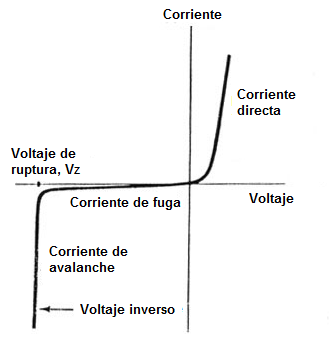
\includegraphics[scale=0.5]{../Ex1/Resources/Diodo}
\par\end{centering}
\caption{Curva de un diodo}
\label{1_6}

\end{figure}

Para resolver este problema de altas frecuencias generadas por los
cambios abruptos, simplemente se añade al circuito un filtro pasivo
de primer orden con comportamiento de pasabajos. Este filtro se logra
con los componentes $C_{3}$ y $R_{x}$, dado que el pasabajos tendrá
una constante de tiempo de establecimiento de $\tau=C_{3}R_{x}$,
estos componentes limitarán el comportamiendo indeseado de los diodos
y mantendran la tensión de gate con pocas variaciones,esto es debido
a la necesidad de controlar muy precisamente la resistencia $R_{DS}$
del transistor. En principio, llamando $f_{0}$ a la frecuencia de
oscilación del oscilador de \emph{Wien }a realizar, se propone que
se cumpla la siguiente inecuación:

\begin{equation}
\frac{1}{f_{0}}<10^{3}C_{3}R_{x}\label{eq:1_3}
\end{equation}

\subsubsection{Controlador de amplitud de oscilación}

Como uno bien se puede imaginar en la subsección \ref{subsec:Diodos-en-serie},
la tensión de umbral entre los diodos determina la tensión máxima
de oscilación del circuito, es decir, para una tensión mayor a la
tensión umbral de ambos diodos, la salida de la sinusoidal se verá
recortada por ese tope de tensión. Para esto, la solución mas intuitiva,
es agregar una caida de tensión variable entre los nodos de los diodos,
para ello, lo unico que se debe hacer es conecta una resistencia variable
en serie con los diodos que genere una caida de tensión variable,
y asi, se podría ajustar el valor máximo de la tension pico de la
señal.

Otra manera un poco mas sofisticada de enfrentar este problema es
agregar un circuito inversor\footnote{Se podría utilizar un circuito no inversor, pero no se lo menciona
ya que no presenta ventajas frente a la resistencia en serie con los
diodos} a la salida del oscilador\footnote{Este método queda a discreción de el presupuesto destinado a realizar
el oscilador.}. La ventaja que se obtiene es que, a diferencia del metodo anterior
donde solo se podia aumentar la tensión máxima de salida, en este
caso, se puede controlar, tanto aumentando la tensión maxima de salida
como atenuandola. El hecho de que invierta la señal no sería un problema
ya que al ser un oscilador la fase de 0\textdegree{} uno la define
donde quiere, por lo tanto, se puede interpretar a la salida con un
defasaje de 0\textdegree . Sin embargo, la gran desventaja de esta
solución es el presupuesto de construcción del mismo, ya que se deben
agregar tanto mas componentes pasivos como activos, y el consumo de
corriente del circuito resultante tambien aumentará debido a la alimentacion
del segundo amplificador. 

Estos dos metodos fueron simulados y los resultados se ven en la Figura
\ref{1_7}.

\begin{figure}[H]
\begin{centering}
\includegraphics[scale=0.5]{\string"../Ex1/Resources/Controlador de amplitud de oscilacion\string".png}
\par\end{centering}
\caption{Cambios en el comportamiendo del circuito para diferentes controladores
de amplitud de oscilación}
\label{1_7}

\end{figure}

\begin{figure}[H]
\begin{centering}
\includegraphics[scale=0.5]{\string"../Ex1/Resources/Circuito Controlador de amplitud por res\string".png}
\par\end{centering}
\caption{Circuito con controlador de amplitud por resistencia}

\end{figure}

\begin{figure}[H]
\begin{centering}
\includegraphics[scale=0.5]{\string"../Ex1/Resources/Circuito Controlador de amplitud por inv\string".png}
\par\end{centering}
\caption{Circuito con controlador de amplitud por etapa inversora}

\end{figure}

\subsection{Máxima frecuencia de oscilación}

Si bien como se ha visto en el análisis anterior, en ningun momento
aparece un limite en la frecuencia de oscilación, esto se debe a que
se trabajó con amplificadores operacionales ideales. Cuando se realiza
el análisis con amplificadores operacionales reales, los limites comienzan
a quedar determinados por el \emph{Gain Bandwidth Product} y el \emph{Slew
Rate. }Al simular el circuito con amplificadores reales, como con
el LM833 o el TL082, se observó que el limite de frecuencias a las
cuales el oscilador dejaba de funcionar dependía del tiempo de establecimiento
que estuvieramos dispuestos a esperar. Es por eso que para tiempos
de establecimiento relativamente razonables, en las simuaciones quedó
en evidencia que que las frecuencias disponibles para realizar el
oscilador no podian superar los 500(kHz).

\subsection{Análisis de sensibilidades}

Se propone calcular analíticamente las sensibilidades del circuito
respecto de los componentes de lazo de realimentación positiva. Para
esto, primero que nada, es necesario calcular la funcion de la realimentación
positiva. Por lo tanto, a continuación se procederá a calcular la
ganancia de realimentación positiva del circuito\footnote{Si bien se podría utilizar la ecuación 10.5 sacada de la pagina 486
del libro, esto no se debe hacer, debido a que en el libro se considera
que $C_{2}$ y $C_{1}$ son iguales, y $R_{2}$ y $R_{1}$ también,
y para el calculo de sensibilidades es necesario considerarlos como
2 componentes distintos.}. Para esto, observando la Figura \ref{1_3}, se plantea por el nodo
$V_{p}$ la siguiente ecuación

\[
\frac{V_{p}-V_{o}}{\frac{1}{sC_{1}}+R_{1}}=-V_{p}\left(sC_{2}+\frac{1}{R_{2}}\right)^{-1}
\]

\begin{equation}
\Rightarrow\beta(s)=\frac{V_{p}}{V_{o}}=\frac{sC_{1}R_{2}}{s^{2}C_{1}C_{2}R_{1}R_{2}+s\left(C_{1}R_{1}+C_{1}R_{2}+C_{2}R_{2}\right)+1}\label{eq:1_4}
\end{equation}

A partir de la ganancia de realimentación positiva de nuestro circuito
calculada en la ecuación \ref{eq:1_4}, de esta manera, operando adecuadamente
con la ganancia del circuito no inversor $(A=1+\frac{R_{3}}{R_{4}})$,
la transferencia de la ecuación \ref{eq:1_2} queda reescrita de la
siguiente manera:

\[
T(s)=\frac{sC_{1}R_{2}\left(1+\frac{R_{3}}{R_{4}}\right)}{s^{2}C_{1}C_{2}R_{1}R_{2}+s\left(C_{1}R_{1}+C_{1}R_{2}+C_{2}R_{2}\right)+1}
\]

Por lo tanto, considerando $C_{1}=C_{2}=C$ y $R_{1}=R_{2}=R$, la
transferencia queda definida como:

\[
\Rightarrow H(s)=\frac{A}{1-T(s)}=\frac{(1+\frac{R_{3}}{R_{4}})\cdot[(sCR)^{2}+s3CR+1]}{(s\cdot CR)^{2}+s\cdot CR(2-\frac{R_{3}}{R_{4}})+1}
\]

Por último, las ecuaciónes de $\omega_{0}$ y \emph{Q }quedan definidas
por:

\begin{equation}
\omega_{0}=\sqrt{\frac{1}{C_{2}R_{2}C_{1}R_{1}}}\label{eq:1_6}
\end{equation}

\[
Q=\frac{\sqrt{C_{1}C_{2}R_{1}R_{2}}}{C_{1}R_{1}+C_{1}R_{2}+C_{2}R_{2}}
\]

De esta manera las sensibilidades quedaran definidas por la formula
\ref{eq:1_5}, y calculando respectivamente cada una de ellas los
resultados son los que se muestran en las ecuaciones posteriores.

\begin{equation}
S_{x_{k}}^{f(\bar{X})}=\left.\frac{\partial f(\bar{X})}{\partial x_{k}}\frac{x_{k}}{f(\bar{X})}\right|_{\bar{X}=\bar{X}_{0}}\label{eq:1_5}
\end{equation}

$S_{C_{1}}^{\omega_{0}}=S_{C_{2}}^{\omega_{0}}=S_{R_{1}}^{\omega_{0}}=S_{R_{2}}^{\omega_{0}}=-\frac{1}{2}$

$S_{C_{1}}^{Q}=-\frac{1}{2}\frac{3C_{1}R_{1}+3C_{1}R_{2}+C_{2}R_{2}}{C_{1}R_{1}+C_{1}R_{2}+C_{2}R_{2}}$

$S_{C_{2}}^{Q}=-\frac{1}{2}\frac{C_{1}R_{1}+C_{1}R_{2}+3C_{2}R_{2}}{C_{1}R_{1}+C_{1}R_{2}+C_{2}R_{2}}$

$S_{R_{1}}^{Q}=-\frac{1}{2}\frac{3C_{1}R_{1}+3CR_{2}+C_{2}R_{2}}{C_{1}R_{1}+C_{1}R_{2}+C_{2}R_{2}}$

$S_{R_{2}}^{Q}=-\frac{1}{2}\frac{C_{1}R_{1}+3C_{1}R_{2}+3C_{2}R_{2}}{C_{1}R_{1}+C_{1}R_{2}+C_{2}R_{2}}$

Si se reemplaza por los valores tal que $C_{1}=C_{2}=C$ y $R_{1}=R_{2}=R$,
entonces los valores de las sensibilidades quedaran como:

\[
S_{C}^{\omega_{0}}=S_{R}^{\omega_{0}}=1
\]

\[
S_{C}^{Q}=S_{R}^{Q}=0
\]

\subsection{Polos y ceros del circuito}

Se procedió a hacer un análisis de los diagramas de polos y ceros
de distintas etapas del circuito para cada situación del mismo.

\section{Implementación}

A lo largo de esta sección nos centraremos en desarrollar el proceso
de implementación del circuito analizado anteriormente. Como primera
etapa, nos centraremos en analizar los componentes que fijan la frecuencia
de oscilación, que es lo primordial en nuestro diseño.

\subsection{Frecuencia de oscilación}

Como se puede observar en la ecuación \ref{eq:1_1_1}, si se toman
valores iguales de $R_{1}=R_{2}=R$ y $C_{1}=C_{2}=C$, entonces con
fijar un valor arbitrariamente, el valor del otro componente quedará
determinado por ese valor, y la frecuencia de operación de nuestro
oscilador. Como nuestra frecuencia de oscilación es de $f_{0}=70\left(kHz\right)$,
fijando el valor del capacitor a un valor comercial conocido, como
$C=10\left(nF\right)$\footnote{Se utilizó este valor para usar los mismos valores que los capacitores
de desacople y obtener un solo valor de capacitor en todo el PCB}, la resistencia por lo tanto quedara fijada y de valor $R=227.36\left(\Omega\right)$.
Debido al hecho de que ese valor de resistencia no es un valor comercial,
se decidió aproximar ese valor al valor comercial más cercano, sea
$R=220(\Omega)$, resultando en un error relativo de resistencia de
$Error\approx3\%$. De esta manera la frecuencia de operación resultante
queda de valor:

\[
f_{0}=72.3\left(kHz\right)
\]

\[
Error\,Relativo=3.34\%
\]

Como se ve en las ecuaciones anteriores, el error relativo de la frecuencia
es demasiado alto, es por esto, que para lograr ajustar la frecuencia
al valor deseado de 70(kHz), si introducirá un preset en el lugar
de la resistencia $R_{2}$, y utilizando la ecuación \ref{eq:1_6},
se la ajustara convenientemente de modo que la frecuencia sea la deseada.
Utilizando este método, se espera obtener un error realtivo de frecuencia
mucho menor, del orden del 0.5\%.

Sin embargo, al recurrir a las simulaciónes se observo que la frecuencia
que se obtenia dadas esas resistencias, era mayor a la obtenida en
la simulación, es por esto, que empiricamente se comprobó que para
llegar a la frecuencia deseada de 70(kHz), era necesario utilizar
resistencias de 195 ohms. Esto fue particularmente bueno ya que se
pueden generar con un paralelo de 2 resistencias de 390 ohms que son
parte del estandard E12 al 1\% de error.

\subsection{\emph{Automatic Amplitude Control (AAC)}}

\subsubsection{Controlador de frecuencia}

Como se mencionó en la sección \ref{subsec:Automatic-Amplitude-Control},
hay varias reglas que se deben tener en cuenta a la hora de sieñar
los valores de los componentes del AAC. En principio, como se propuso
en la inecuación \ref{eq:1_3}, se decide tomar el capacitor $C_{3}=10(nF)$,
para utilizar solo un tipo de valor de capacitor en todo nuestro circuito,
y por ende, el valor de la resistencia quedará fijo en $R_{x}>285.71\Omega$.
Por ende, para lograr una buena relación entre impedancias, se eligió
un valor de $R_{x}=10(k\Omega)$.

\subsubsection{Elección de la resistencia del transistor JFET-N}

Debido a las relaciones mencionadas en la sección \ref{subsec:Diodos-en-serie},
se deben cumplir ciertas relaciónes entre las resistencias $R_{3}$,
$R_{4}$ y $R_{T}$, estas relaciones (que fueron explicadas anteriormente),
quedan sintetizadas en las siguientes expresiones:

\[
\left\{ \begin{array}{c}
\frac{R_{3}}{R_{4}}=K_{1}\\
\frac{R_{3}}{R_{4}+R_{T}}=K_{2}
\end{array}\right.
\]

\[
K_{1}>2\,\,;\,\,K_{2}<2
\]

Debido a que se elige un tiempo de establecimiento del oscilador relativamente
corto, se elige arbitrariamente $K_{1}=2.2$ y $K_{2}=1.8$, mateniendo
simetría entre ambas constantes y siendo lo suficintemente dstantes
del 2 como para ajustar rapidamente cualquier variación respecto del
2. Como se puede observar en la Figura \ref{1_5}, el valor de la
resistencia del transistor $R_{T}$, varia dependiendo de la polarización
del mismo, es or esto, que se elige polarizarlo con la mayor resistencia
posible. Por esta razon, y como se puede ver en la figura, la impedancia
del transistor varía abruptamente para valores entre 0 y 3 (mV) de
$V_{GS}$, es por esto que vamos a considerar esta resistencia como
$0(\Omega)$ cuando el transistor se encuentre apagado y como $\sim550(\Omega)$
cuando el transistor se encuentra encendido. Por lo tanto $R_{T}\approx550(\Omega)$,
por ende los valores de las otras resistencias quedarán bien determinadas
por los valores:

$R_{3}=5.4(k\Omega)$

$R_{4}=2.4(k\Omega)$

Si bien estos valores son correctos, solo falta ajustarlos de manera
que se encuentren dentro de valores comerciales de resistencias, es
por eso que se los implementará con resistencias en resie y paralelo
para llegar a un valor lo más cercano posible.

\subsubsection{Polos y ceros}

Por lo tanto, teniendo ya definidos estos valores a utilizar, ya es
posible realizar un diagrama de polos y ceros del circuito, estos
se pueden observar en las Figuras .
\begin{center}
\begin{figure}[H]
\begin{centering}
\subfloat[Sin la resistencia del transistor]{\begin{centering}
\includegraphics[scale=0.4]{\string"../Ex1/Resources/PolosYCeros para lazo abierto SIN TRANS\string".png}
\par\end{centering}
}\subfloat[Con la resistencia del transistor]{\begin{centering}
\includegraphics[scale=0.4]{\string"../Ex1/Resources/PolosYCeros para lazo abierto CON TRANS\string".png}
\par\end{centering}

}
\par\end{centering}
\begin{centering}
\caption{Diagrama de polos y ceros para la ganancia de lazo}
\par\end{centering}
\end{figure}
\par\end{center}

\begin{center}
\begin{figure}[H]
\begin{centering}
\subfloat[Sin la resistencia del transistor]{\begin{centering}
\includegraphics[scale=0.4]{\string"../Ex1/Resources/PolosYCeros para H SIN TRANS\string".png}
\par\end{centering}

}\subfloat[Con la resistencia del transistor]{\begin{centering}
\includegraphics[scale=0.4]{\string"../Ex1/Resources/PolosYCeros para H CON TRANS\string".png}
\par\end{centering}

}
\par\end{centering}
\centering{}\caption{Diagrama de polos y ceros para la transferencia del circuito}
\end{figure}
\par\end{center}

\subsection{Selección de amplificadores operacionales}

Para la seleccion del amplificador operacional a utilizar, se tuvieron
en cuenta solo aquellos que se encontraban disponibles al dia de la
fecha de imlementación del circuito en el pañol de la universidad.
Esto se debe, a que en trabajos prácticos anteriores, esto no fue
tenido en cuenta y a la hora de implementar el circuito fue necesario
realizar muchos cambios debido a esto. Los amplificadores disponibles
en el pañol y sus respectivas características se pueden observar en
el cuadro \ref{1_8}.

\begin{table}[h]
\begin{centering}
\begin{tabular}{|c|c|c|c|c|c|}
\hline 
Amplificador & GBP & $A_{Vol}$ & \emph{Slew Rate} & $Z_{in}$ & THD\tabularnewline
\hline 
\hline 
TL082 & 3(MHz) & 200$\left(\frac{V}{mV}\right)$ & $13(\frac{V}{\mu s})$ & $10^{12}(\Omega)$ & <0.0003\tabularnewline
\hline 
TL072 & 3(MHz) & 200$\left(\frac{V}{mV}\right)$ & $13(\frac{V}{\mu s})$ & $10^{12}(\Omega)$ & <0.0003\tabularnewline
\hline 
LM741 & 1.5(MHz) & 200$\left(\frac{V}{mV}\right)$ & $0.5(\frac{V}{\mu s})$ & $2^{6}(\Omega)$ & <0.0006\tabularnewline
\hline 
\end{tabular}
\par\end{centering}
\caption{Características de amplificadores operacionales disponibles}
\label{1_8}
\end{table}

Viendo esos valores y utilizando la ecuación (\ref{eq:1_7}) de selección
propuesta\footnote{A mayor valor, mejor es el opamp analizado}, se
obtiene que para esos valores de ponderación, el amplificador operacional
optimo a utilizar es el TL082 o igualmente el TL072\footnote{Los valores obtenidos con la ecuación dan como resultado que ambos
operacionales son igual de capaces para los valores de ponderación
propuestos, sin embargo, se decidió utilizar el TL82 debido a que
es un integrado mas pequeño y por ende el desarrollo del PCB queda
mas compacto.}.

\begin{equation}
Valor=\frac{GBP}{10\cdot10^{6}}\cdot0.5+\frac{A_{Vol}}{100}\cdot0.2+\frac{SR}{10}\cdot0.1+\frac{Z_{in}}{10^{12}}\cdot0.1+\frac{THD}{10^{-4}}\cdot0.1\label{eq:1_7}
\end{equation}

tl082 2.43

lm741 1.755

\subsection{Diseño del PCB}

Por ultimo, el PCB implementado desarrollado con el programa \emph{Altium
Designer}, quedo como se pueden ver en las Figuras \ref{1_10} y \ref{1_11}.

\begin{figure}[H]
\begin{centering}
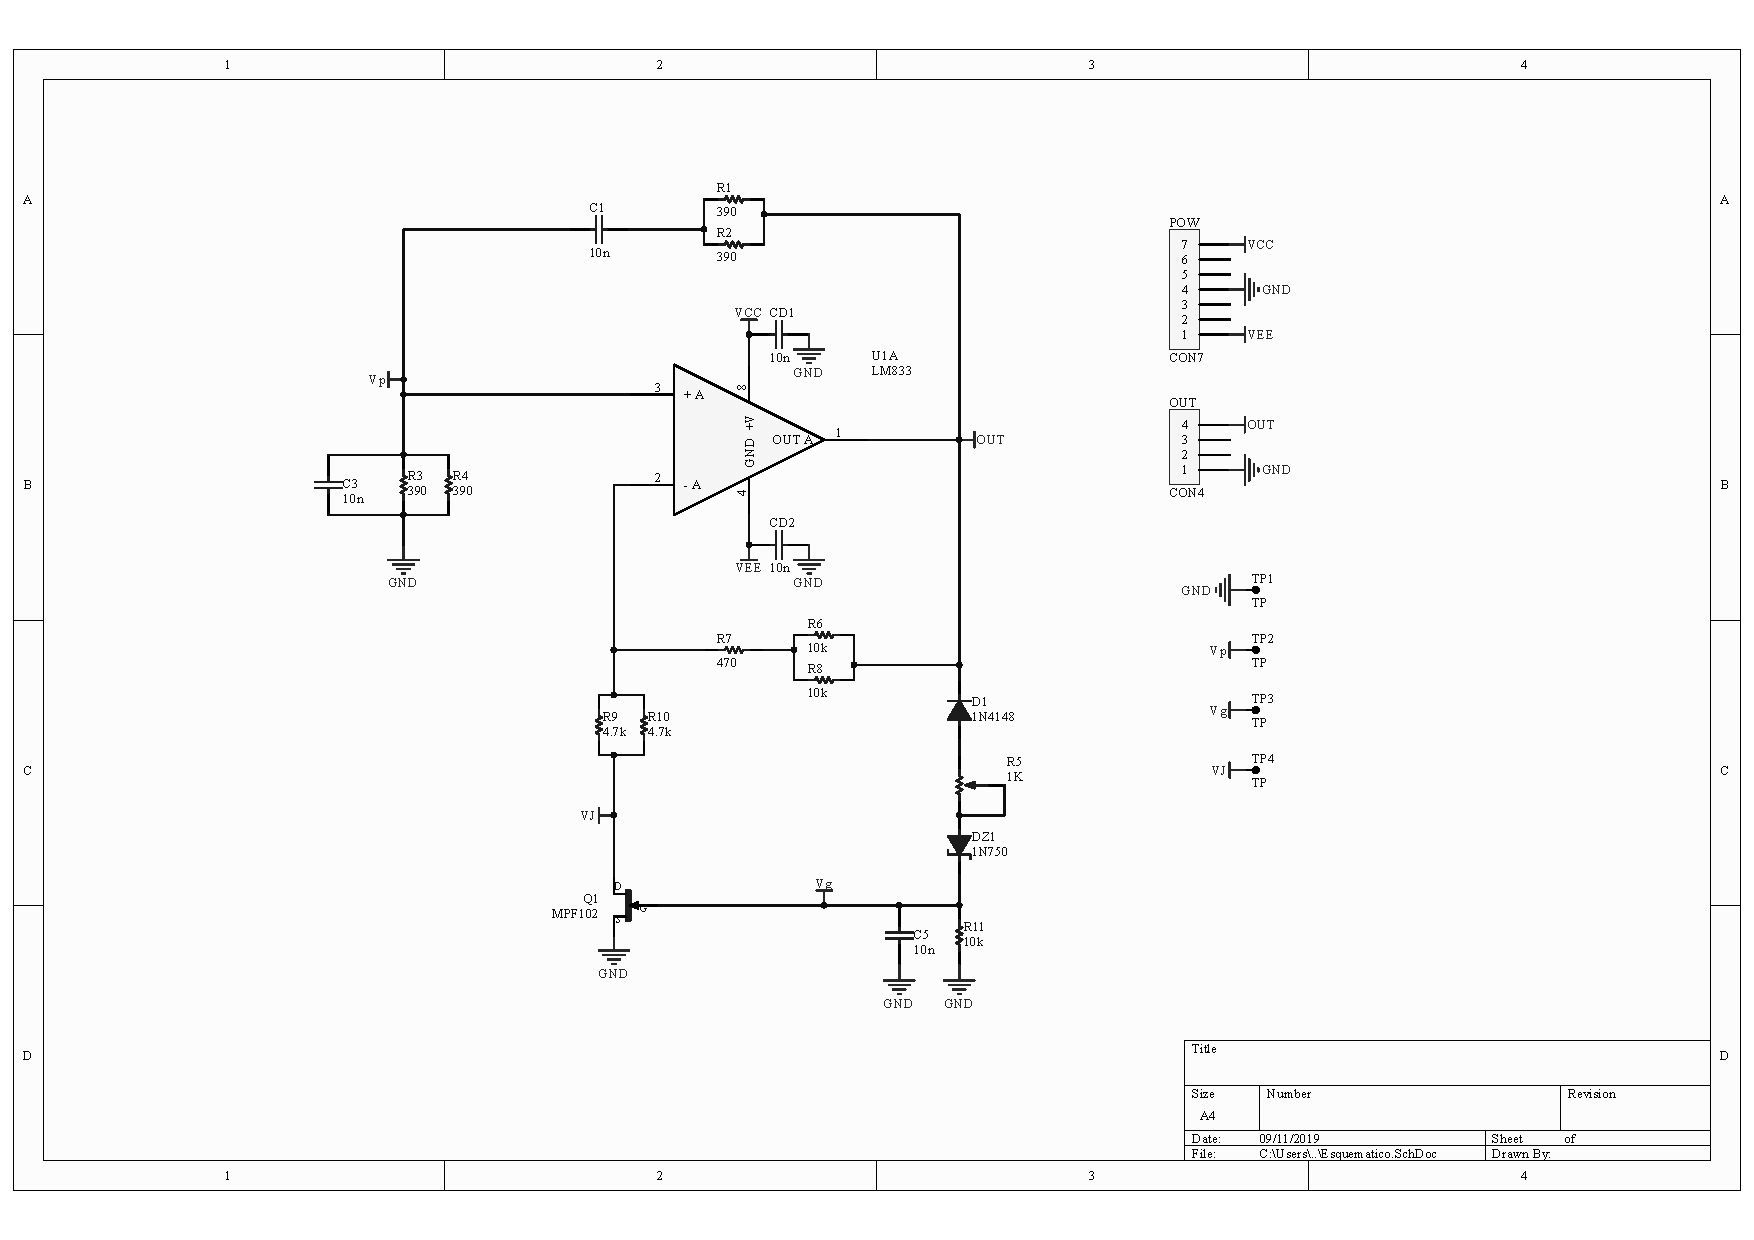
\includegraphics[scale=0.5]{../Ex1/Resources/Esquematico}
\par\end{centering}
\caption{Esquemático}

\label{1_10}
\end{figure}

\begin{figure}[H]
\begin{centering}
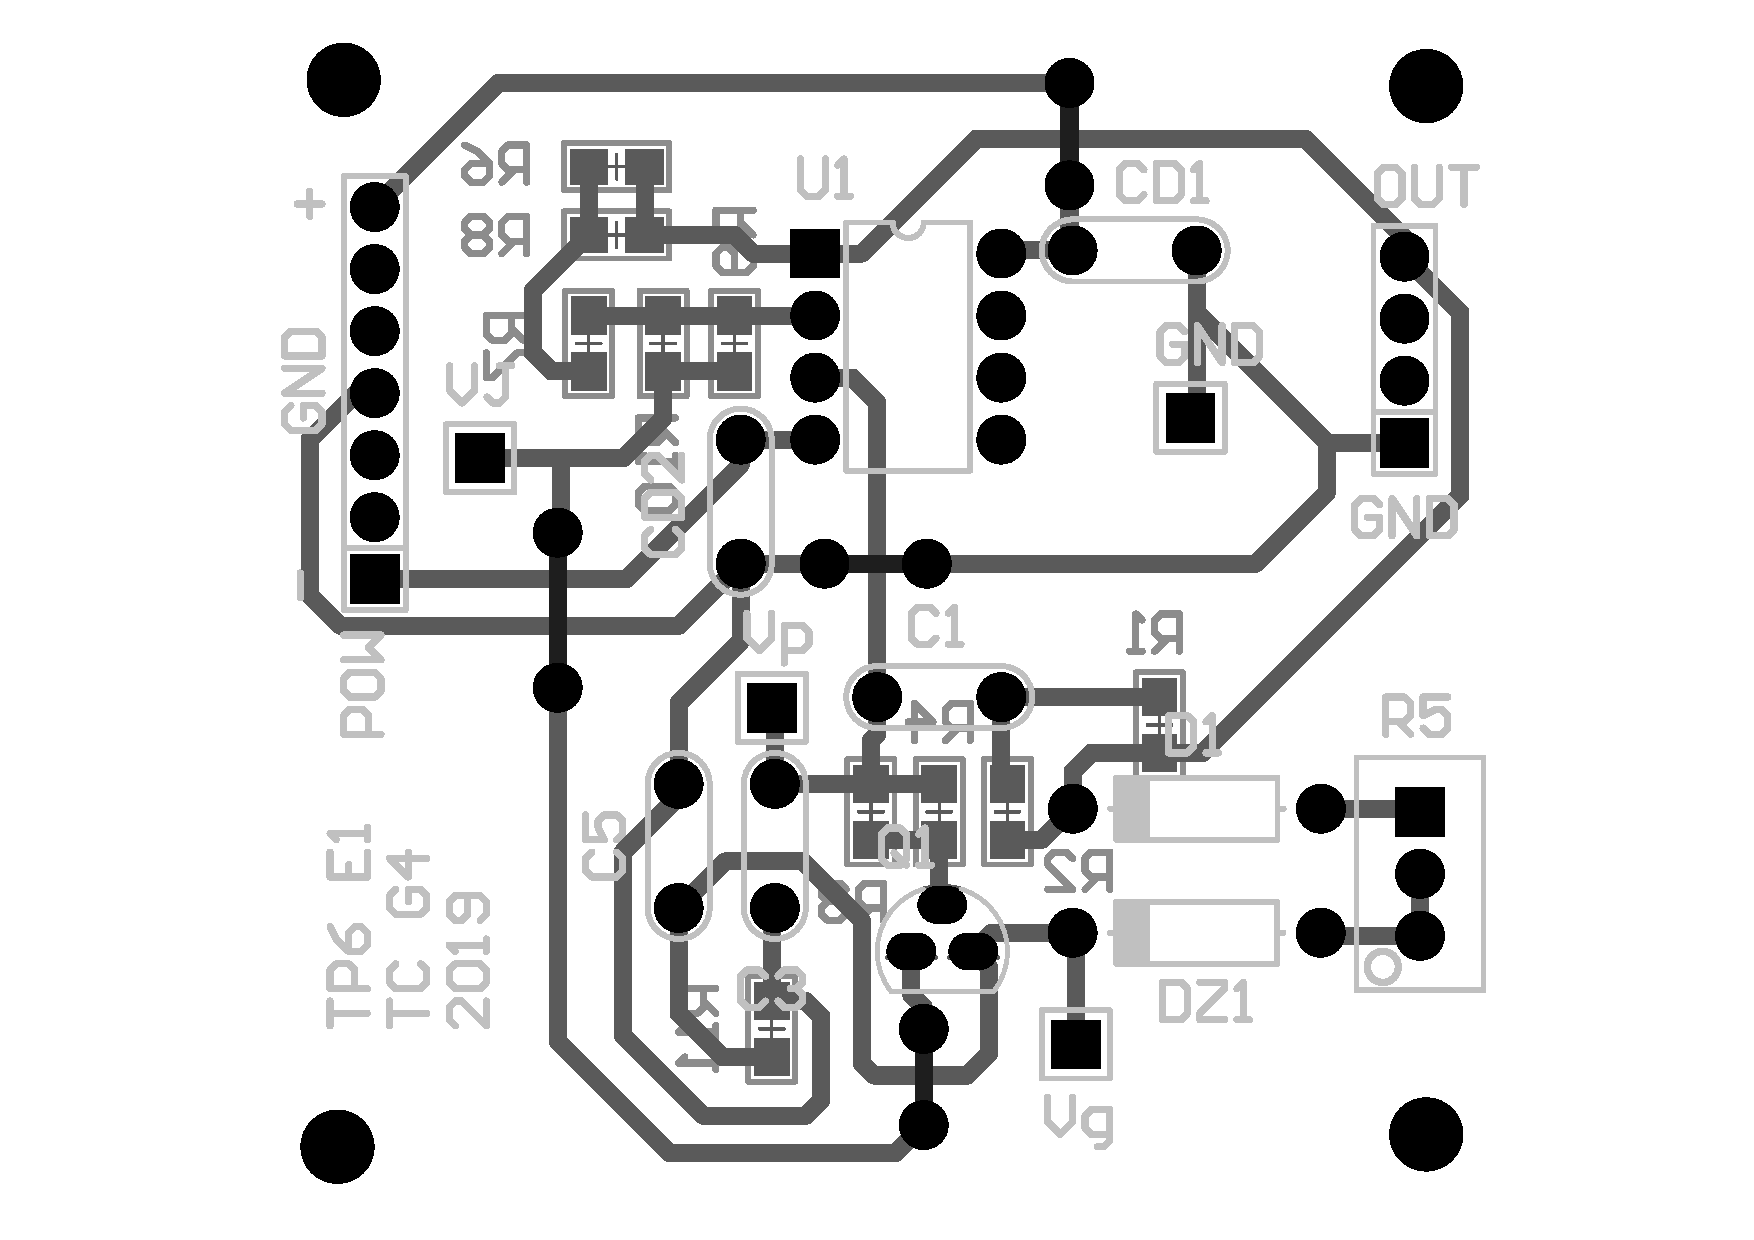
\includegraphics[scale=0.25]{../Ex1/Resources/PCB}
\par\end{centering}
\caption{PCB}
\label{1_11}

\end{figure}

\section{Simulaciones y mediciones}

A lo largo de esta sección nos centraremos en realizar las simulaciones
pertinentes del circuito y las mediciones del mismo. En la Figura
\ref{1_16}, se puede observar una simulación y medición del circuito
funcionando.

\begin{figure}[H]
\begin{centering}
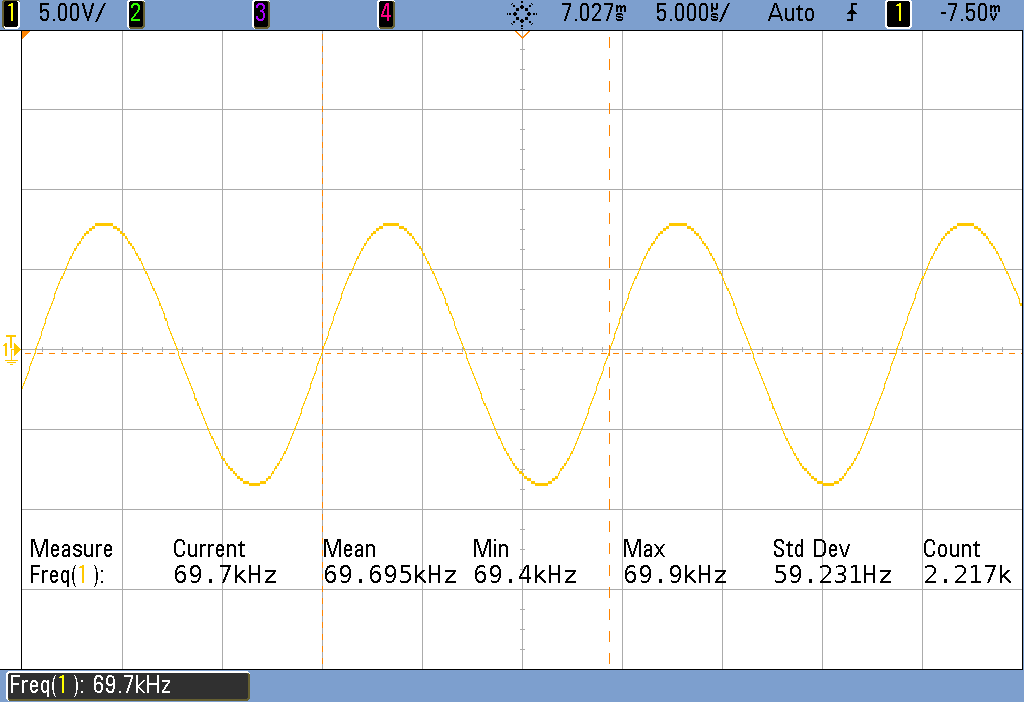
\includegraphics[scale=0.35]{../Ex1/Resources/Oscilacion}
\par\end{centering}
\caption{Oscilación del circuito}
\label{1_16}

\end{figure}

\subsection{Distorsión Armónica}

Debido a imperfecciones propias de la realidad, la generación de señales
senoidales completamente puras es imposible. Es por ello que es necesario
realizar un análisis de cuantá es la distorsión armonica de nuestro
oscilador. Para realizar estos análisis se hace uso del llamado \emph{Total
Harmonic Distortion, }que es un parámetro que da cuenta de cuanto
esta distorsionada nuestra señal respecto al armónico principal. Si
realizamos una \emph{Fast Fourier Transform} (FFT) a la señal generada
por el oscilador, podemos observar mas detalladamente la componente
de potencia que tienen todos los armonicos de la señal, esta imagen
se puede observar en la Figura \ref{1_12}. Como se puede observar,
es notorio que cuanto mas grande sea el armonico, mas atenuado estará.

\begin{figure}[H]
\begin{centering}
\includegraphics[scale=0.5]{\string"../Ex1/Resources/FFT SIMULADO\string".png}
\par\end{centering}
\caption{FFT de la señal generada}
\label{1_12}

\end{figure}

Si se mide la potencia de los primeros 5 armónicos siguientes al armonico
principal, la distorsión armónica da como resultado lo siguiente:

\[
THD=0.0206
\]

Por otro lado, al medir el espectro en frecuencia de la señal con
una FFT en el osciloscopio, el resultado fue el que se muestra en
la Figura \ref{1_13}.

\begin{figure}[H]
\begin{centering}
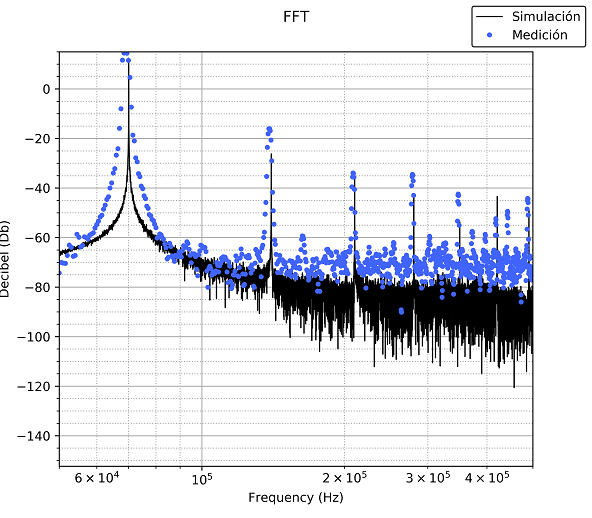
\includegraphics[scale=0.7]{../Ex1/Resources/FFT}
\par\end{centering}
\caption{FFT de la señal generada}
\label{1_13}

\end{figure}

Donde se puede observar que la distorsión armónica es prácticamente
igual a la simulada.

\subsection{Transistor en estado estacionario}

\subsubsection{Resistencia dinámica}

Luego de que se llego al estado estacionario del circuito, es decir
cuando termino el tiempo transitorio desde que se lo conecto a una
fuente, la resistencia dinámica del transistor debería quedar en un
valor, de tal manera que la relación de impedancias $\frac{R_{3}}{R_{4}+R_{T}}=2$,
para esto, despejando de los valores de las reistencias, $R_{T}$
deberia tener un valor cercano a $300(\Omega)$. Esto se verifica
al ver la Figura \ref{1_14}, que muestra la simulación hecha con
LTSpice.

\begin{figure}[H]
\begin{centering}
\includegraphics[scale=0.7]{\string"../Ex1/Resources/Resistencia transistor SIMULADO\string".png}
\par\end{centering}
\caption{Simulación de resistencia del transistor en el estado estacionario}
\label{1_14}

\end{figure}

\subsubsection{Tensión de Gate}

Para lograr obtener los valores de resistencia aproximadamente dentro
del rango requerido, es necesario que la tensión de gate a su vez
tenga pequeñas variaciones cerca de un intervalo. Si se simula la
tensión de gate en el estado estacionario, el resultado se puede observar
en la Figura \ref{1_15}.

\begin{figure}[H]
\begin{centering}
\includegraphics[scale=0.6]{\string"../Ex1/Resources/Tension de gate SIMULADA\string".png}
\par\end{centering}
\caption{Tensión de gate en el estado estacionario}

\label{1_15}
\end{figure}

\begin{figure}[H]
\begin{centering}
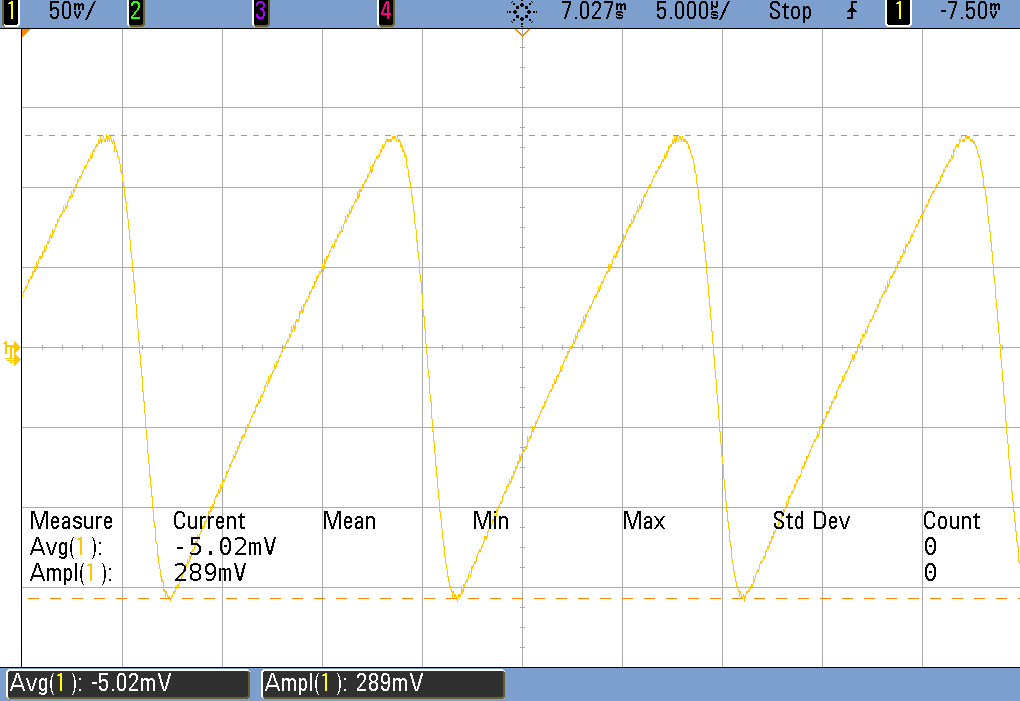
\includegraphics[scale=0.35]{../Ex1/Resources/VG}
\par\end{centering}
\caption{Medición de la tensión de gate}

\end{figure}

Como se puede observar, la tensión de gate tiene variaciones máximas
de 0.2(mV), por lo cual, a fines prácticos, y considerando el ruido
electromagnético de laboratorio, se la puede considerar constante.
